% IEEE conference version for GTSD 2026 proceedings
\documentclass[conference]{IEEEtran}
\usepackage{cite}
\usepackage{amsmath,amssymb,amsfonts}
\usepackage{graphicx}
\graphicspath{{figures/}}
\usepackage{textcomp}
\usepackage{booktabs}
\usepackage{algorithm}
\usepackage{algpseudocode}
\usepackage{url}
\def\BibTeX{{\rm B\kern-.05em{\sc i\kern-.025em b}\kern-.08em
    T\kern-.1667em\lower.7ex\hbox{E}\kern-.125emX}}

\begin{document}
\bstctlcite{IEEEexample:BSTcontrol}

% Initialize section counter to 2 so this section compiles cleanly as Section III (Part 1: III-A, III-B, III-C)
\setcounter{section}{2}

\section{Proposed Hardware-Software Co-Design Framework}

% =========================================================================
% III-A. OVERALL SYSTEM ARCHITECTURE & CO-DESIGN WORKFLOW
% =========================================================================
\subsection{Overall System Architecture and HW/SW Co-Design Workflow}

Deploying deep super-resolution models on resource-constrained edge modalities presents a fundamental architectural dilemma: general-purpose embedded CPUs lack the parallel arithmetic throughput required for real-time 2D convolutions, whereas purely autonomous FPGA implementations suffer from severe development overhead regarding peripheral interfacing, file I/O, and dynamic memory orchestration. To overcome these constraints, we establish a balanced, end-to-end hardware-software co-design architecture deployed on the heterogeneous Xilinx Zynq-7020 System-on-Chip (SoC) \cite{kalapothas2022efficient, pynqhomepage}. As illustrated in Fig.~\ref{fig:sw_hw_architecture}, the system is partitioned into two synchronized computing domains across distinct clock regimes: (1) the software-driven \textbf{Processing System (PS)} running at 650~MHz, and (2) the custom pipelined \textbf{Programmable Logic (PL)} streaming accelerator core operating at a deterministic clock rate of 100~MHz.

\begin{figure*}[t]
\centering
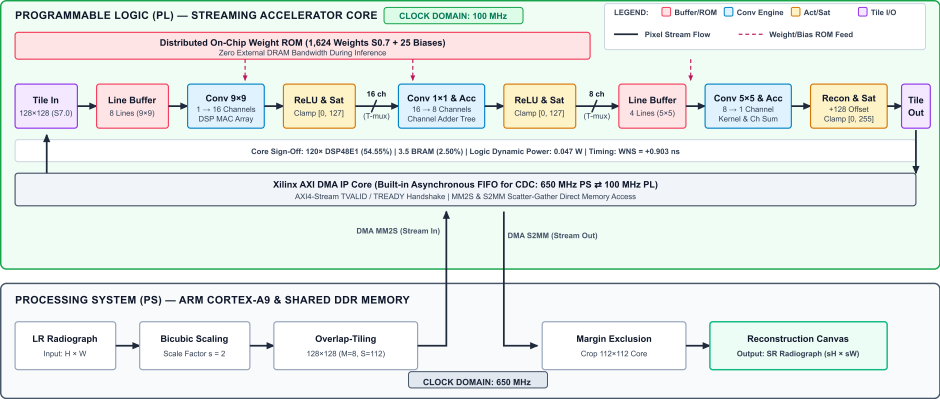
\includegraphics[width=\textwidth]{SW-HW_architeture.jpg}
\caption{End-to-end heterogeneous hardware-software co-design architecture: (1) Processing System (PS) domain running on dual-core ARM Cortex-A9 (650~MHz) for bicubic scaling, overlap-tiling partitioning ($128 \times 128$, $M=8, S=112$), margin exclusion, and final frame stitching, and (2) Programmable Logic (PL) streaming accelerator core (100~MHz) incorporating on-chip distributed weight ROM (1,624 weights S0.7 + 25 biases), 2D line buffers, parallel DSP MAC arrays, and pipelined channel adder trees, interfaced via Xilinx AXI DMA with built-in asynchronous FIFO clock-domain crossing (CDC).}
\label{fig:sw_hw_architecture}
\end{figure*}

\subsubsection{Processing System (PS) Workflow: Pre-Processing and Canvas Reconstruction}
The Processing System (PS), powered by a dual-core ARM Cortex-A9 processor running at 650~MHz under the embedded Linux/PYNQ environment \cite{pynqhomepage}, coordinates high-level medical radiograph management, coordinate geometry transformations, and DMA buffer allocation:
\begin{itemize}
    \item \textbf{Bicubic Scaling:} Given an input low-resolution (LR) radiograph $I_{LR} \in \mathbb{R}^{H \times W}$, the host CPU executes software-based bicubic interpolation by an upscaling factor of $s = 2$, mapping the image onto the target high-resolution (HR) spatial grid ($2H \times 2W$). This pre-upsampling establishes a spatially uniform dataflow for subsequent convolutional stages.
    \item \textbf{Overlap-Tiling Partitioning:} To accommodate the limited on-chip memory budget of edge FPGAs, the interpolated frame is partitioned into overlapping tiles of dimension $P \times P = 128 \times 128$ pixels, using an effective core stride of $S = 112$ and a boundary margin of $M = 8$. Each patch is formatted into signed 8-bit fixed-point representation (S7.0, range $[-128, 127]$).
    \item \textbf{Margin Exclusion and Stitching:} Once super-resolved tiles return from the hardware accelerator, the PS software pipeline discards the $M = 8$ exterior border pixels affected by valid convolution boundary shrinkage, isolating the artifact-free $112 \times 112$ core ($T_{valid}$). The valid cores are subsequently stitched into a continuous reconstruction canvas to reconstruct the full diagnostic radiograph ($I_{SR} \in \mathbb{R}^{sH \times sW}$).
\end{itemize}

\subsubsection{Clock-Domain Crossing and AXI DMA IP Interconnect}
Data interchange between the 650~MHz Processing System and the 100~MHz Programmable Logic fabric is arbitrated by an on-chip \textbf{Xilinx AXI Direct Memory Access (AXI DMA) IP Core}. The DMA controller bridges the two asynchronous clock domains using built-in asynchronous dual-clock FIFOs, completely eliminating metastability risks and clock-domain crossing (CDC) penalties. Utilizing high-throughput 64-bit AXI High-Performance (HP) ports, the DMA engine performs bidirectional Scatter-Gather streaming:
\begin{itemize}
    \item \textbf{DMA MM2S Channel (\textit{Memory-Mapped to Stream}):} Reads contiguous S7.0 input tile buffers directly from off-chip DDR3 DRAM and streams them into the accelerator's AXI4-Stream Slave port under standard \texttt{TVALID}/\texttt{TREADY} flow control.
    \item \textbf{DMA S2MM Channel (\textit{Stream to Memory-Mapped}):} Captures the super-resolved output stream from the accelerator's AXI4-Stream Master port, automatically transferring completed frames into destination memory upon detecting the asserted \texttt{TLAST} packet boundary flag.
\end{itemize}

\subsubsection{Programmable Logic (PL) Streaming Accelerator Datapath}
The custom hardware accelerator instantiated on the Artix-7 logic fabric of the Zynq-7020 executes the entire 3-layer compact SRCNN inference pipeline in a continuous streaming manner at 100~MHz:
\begin{itemize}
    \item \textbf{Distributed On-Chip Weight ROM:} All 1,624 quantized convolutional weights (signed S0.7) and 25 biases are pre-loaded into distributed on-chip ROM blocks directly adjacent to the compute cores. This architectural choice achieves \textit{zero external DRAM memory bandwidth during active inference}, entirely circumventing the von Neumann memory wall \cite{sze2017efficient}.
    \item \textbf{Layer 1 (Patch Extraction \& Feature Representation):} Streaming S7.0 pixels pass through an 8-line 2D line buffer (BRAM-based shift registers) that reconstructs a full $9 \times 9$ spatial sliding window on every clock cycle. The $9 \times 9$ convolution engine employs a parallel DSP MAC array to project the single input channel into 16 intermediate feature maps ($1 \rightarrow 16$), followed by a parametric ReLU and saturation unit that clamps activations into $[0, 127]$. The resulting 16 channels are time-multiplexed (\textit{T-mux}) into the next stage.
    \item \textbf{Layer 2 (Non-linear Mapping):} A $1 \times 1$ convolution engine paired with a balanced, pipelined channel adder tree compresses the 16 feature maps into 8 channels ($16 \rightarrow 8$). Activations are clamped via a second ReLU and saturation stage before being time-multiplexed into the final reconstruction layer.
    \item \textbf{Layer 3 (High-Resolution Reconstruction):} The 8-channel activations enter a 4-line buffer to form a $5 \times 5$ sliding window. The $5 \times 5$ convolution engine ($8 \rightarrow 1$) computes both spatial kernel products and multi-channel accumulations concurrently. The final Reconstruction \& Saturation block adds a $+128$ offset to de-quantize signed intermediate values back to standard unsigned uint8 representations ($[0, 255]$), streaming the super-resolved tile out via the AXI4-Stream Master interface.
    \item \textbf{Hardware Sign-Off Summary:} The accelerator core achieves complete timing closure with a positive Worst Negative Slack of $\text{WNS} = +0.903$~ns at 100~MHz, while consuming merely 120 DSP48E1 slices (54.55\% of budget), 3.5 BRAM blocks (2.50\%), and dissipating an ultra-low logic dynamic power of only 0.047~W.
\end{itemize}

The subsequent subsections detail the mathematical formulation of the compact network topology (Section~\ref{sec:topology}), the fixed-point quantization scheme (Section~\ref{sec:quantization}), the boundary-safe overlap-tiling strategy (Section~\ref{sec:tiling}), and the internal microarchitectural timing closure (Section~\ref{sec:rtl_arch}).

% =========================================================================
% III-B. COMPACT SRCNN NETWORK TOPOLOGY & TRAINING PROTOCOL
% =========================================================================
\subsection{Compact SRCNN Network Topology and Pre-Quantization Training}
\label{sec:topology}

To achieve deterministic throughput and meet the rigorous resource boundaries of the Xilinx Zynq-7020 SoC, we formulate a hardware-tailored, compact 3-layer Convolutional Neural Network based on the pre-upsampling SRCNN paradigm. Unlike post-upsampling models (such as FSRCNN \cite{dong2016accelerating} or ESPCN \cite{shi2016real}) that introduce irregular transposed zero-insertion or multi-clock domain spatial shuffling logic, pre-upsampling maintains identical spatial resolutions across all intermediate feature maps. This structural regularity enables a single-rate streaming line-buffer topology without pipeline stalls.

\begin{figure}[t]
\centering
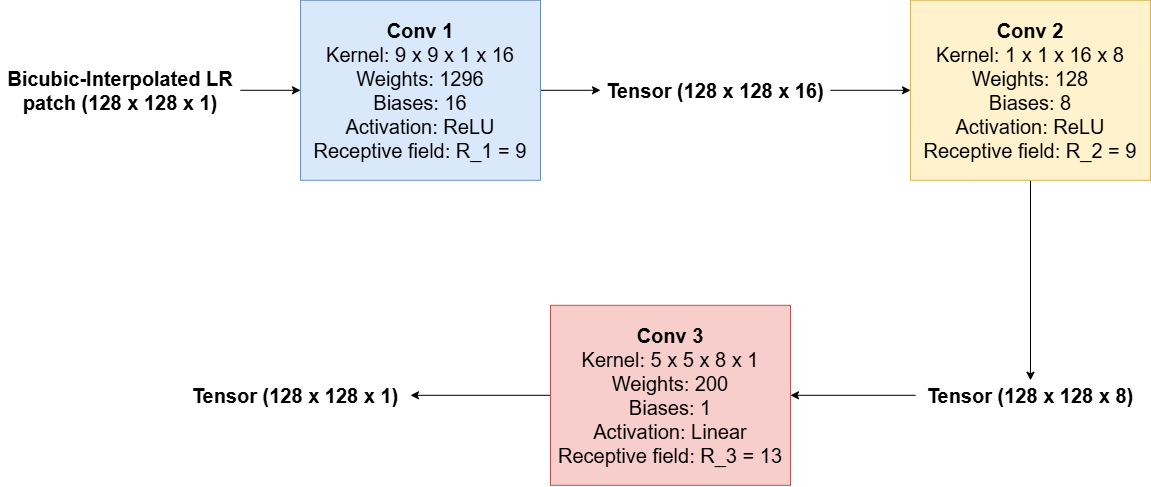
\includegraphics[width=\columnwidth]{compact_srcnn_topology.png}
\caption{Architectural topology and tensor dimensions of the proposed compact 3-layer SRCNN ($1 \rightarrow 16 \rightarrow 8 \rightarrow 1$). The network extracts 16 feature maps via a $9 \times 9$ kernel, compresses representations to 8 channels using a pointwise $1 \times 1$ mapping, and reconstructs the target radiograph via a $5 \times 5$ spatial synthesis filter, totaling 1,649 parameters with a cumulative receptive field of 13 pixels.}
\label{fig:network_topology}
\end{figure}

\subsubsection{Layer-by-Layer Architectural Formulation}
The original SRCNN proposed by Dong \textit{et al.} \cite{dong2014learning} incorporates a $64 \rightarrow 32$ channel configuration with 8,032 weights, requiring excessive parallel Multiply-Accumulate (MAC) resources for low-cost edge FPGAs. We design a slimmed $1 \rightarrow 16 \rightarrow 8 \rightarrow 1$ topology that preserves high clinical reconstruction fidelity while drastically reducing hardware footprint, as illustrated in Fig.~\ref{fig:network_topology}:
\begin{enumerate}
    \item \textbf{Layer 1 --- Patch Extraction and Representation:} The input is an interpolated single-channel grayscale patch $Y \in \mathbb{R}^{H \times W \times 1}$. Layer~1 applies 16 spatial filters of size $9 \times 9 \times 1$, parameterized by weight tensor $W_1 \in \mathbb{R}^{9 \times 9 \times 1 \times 16}$ and bias vector $B_1 \in \mathbb{R}^{16}$. This operation extracts high-dimensional localized spatial features and is activated by a Rectified Linear Unit (ReLU):
    \begin{equation}
    F_1(Y) = \max\left(0,\, W_1 * Y + B_1\right)
    \label{eq:layer1_conv}
    \end{equation}
    The weight footprint of this stage is $9 \times 9 \times 1 \times 16 = 1,296$ weights and 16 biases.
    
    \item \textbf{Layer 2 --- Non-linear Mapping:} The 16-channel feature tensor $F_1(Y)$ is mapped to an 8-channel latent representation via a pointwise $1 \times 1$ convolution, governed by weights $W_2 \in \mathbb{R}^{1 \times 1 \times 16 \times 8}$ and biases $B_2 \in \mathbb{R}^{8}$:
    \begin{equation}
    F_2(Y) = \max\left(0,\, W_2 * F_1(Y) + B_2\right)
    \label{eq:layer2_conv}
    \end{equation}
    Layer~2 introduces non-linear cross-channel interactions with minimal computational overhead ($1 \times 1 \times 16 \times 8 = 128$ weights and 8 biases), acting as an efficient dimensional bottleneck.
    
    \item \textbf{Layer 3 --- High-Resolution Reconstruction:} The final layer aggregates the 8-channel intermediate representations using a $5 \times 5 \times 8 \times 1$ convolutional kernel, parameterized by $W_3 \in \mathbb{R}^{5 \times 5 \times 8 \times 1}$ and scalar bias $B_3 \in \mathbb{R}^{1}$:
    \begin{equation}
    F_3(Y) = W_3 * F_2(Y) + B_3
    \label{eq:layer3_conv}
    \end{equation}
    Crucially, Layer~3 produces a strictly linear output without ReLU activation. Omitting non-linear thresholding at the reconstruction stage prevents the clipping of negative residual details, ensuring full preservation of the diagnostic radiological contrast range in bone structures and soft lung tissues. This stage consumes $5 \times 5 \times 8 \times 1 = 200$ weights and 1 bias.
\end{enumerate}

Across the three layers, the compact network comprises exactly $1,296 + 128 + 200 = 1,624$ convolutional weights and $16 + 8 + 1 = 25$ biases, establishing an ultra-compact parameter footprint of $1,649$ total parameters. This achieves a $79.8\%$ weight reduction (1,624 vs. 8,032 weights) and a $79.7\%$ total parameter reduction (1,649 vs. 8,129 parameters) compared to baseline SRCNN \cite{dong2014learning}.

\subsubsection{Pre-Quantization Training Protocol}
To establish an optimal full-precision (FP32) baseline prior to fixed-point hardware quantization, the network is trained using clinical radiographs. We extract 15,000 sub-patches of size $64 \times 64$ pixels from the clinical training split. High-resolution reference patches $X_i$ and low-resolution inputs $Y_i$ (downscaled by factor $s = 2$ and pre-interpolated to match $X_i$) form paired training observations.

Because convolutional operations are inherently translation-invariant and patch-size-agnostic, training on smaller $64 \times 64$ sub-patches accelerates backpropagation convergence, mitigates GPU memory footprint, and maximizes effective spatial augmentation variety across heterogeneous chest anatomies. Conversely, deploying on larger $128 \times 128$ tiles during FPGA inference maximizes the area ratio of the valid reconstructed core to the boundary margin ($112^2 / 128^2 = 76.56\%$), substantially amortizing line-buffer flushing overhead and DMA transfer transactions.

Rather than employing standard Mean Squared Error ($L_2$ loss), which is known to cause structural over-smoothing and penalize diagnostic sharpness, we optimize the network parameters $\theta = \{W_1, W_2, W_3, B_1, B_2, B_3\}$ using the Charbonnier loss function \cite{charbonnier1994two} (a differentiable approximation of the $L_1$ norm):
\begin{equation}
\mathcal{L}(\theta) = \frac{1}{N} \sum_{i=1}^N \sqrt{\| F_3(Y_i; \theta) - X_i \|^2 + \epsilon^2}
\label{eq:charbonnier_loss}
\end{equation}
where $\epsilon = 10^{-3}$ ensures numerical stability. The optimization is conducted using the Adam optimizer \cite{kingma2014adam} with momentum coefficients $\beta_1 = 0.9$ and $\beta_2 = 0.999$. The initial learning rate is set to $\eta = 10^{-3}$ and modulated via a cosine annealing schedule over 50 training epochs with a mini-batch size of 64. 

This training regimen achieves a floating-point reconstruction fidelity of 39.31~dB PSNR and 0.9602 SSIM on unseen test radiographs. This high baseline fidelity ensures that subsequent 8-bit post-training quantization introduces negligible performance degradation ($<0.04$~dB PSNR loss), directly yielding the verified 39.278~dB PSNR and 0.9598 SSIM hardware-deployed performance.

% =========================================================================
% III-C. FIXED-POINT MATHEMATICAL FORMULATION & POST-TRAINING QUANTIZATION
% =========================================================================
\subsection{Fixed-Point Mathematical Formulation and Post-Training Quantization (PTQ Q7)}
\label{sec:quantization}
\label{sec:ptq}

Deploying deep neural networks in standard IEEE-754 single-precision floating-point (FP32) arithmetic incurs prohibitive hardware overhead on edge-class FPGAs. Floating-point multipliers and adders demand expansive look-up table (LUT) logic and induce deep pipeline latencies that limit clock frequencies. To maximize compute density, minimize on-chip routing congestion, and comply with the strict thermal budget of the Xilinx Zynq-7020 SoC, we formulate an exact 8-bit signed fixed-point Post-Training Quantization scheme \cite{jacob2018quantization, sze2017efficient}, denoted as \textbf{PTQ Q7}.

\subsubsection{Data Representation: S7.0 and S0.7 Number Formats}
We adopt two complementary signed 8-bit fixed-point representations, following the standard notation $\text{S}(I.F)$, where $\text{S}$ denotes the 2's-complement sign bit, $I$ is the number of integer bits, and $F$ is the number of fractional bits ($1 + I + F = 8\text{ bits}$):
\begin{itemize}
    \item \textbf{Pixel Activations ($\text{S7.0}$):} Feature activations across all convolutional layers are represented as signed 8-bit integers with 7 integer bits and 0 fractional bits ($I=7, F=0$). This format spans the discrete dynamic range $[-128,\, 127]$ with a unit step size of $\Delta_X = 1.0$.
    \item \textbf{Model Weights ($\text{S0.7}$):} Because convolutional weight distributions in our trained model are tightly bounded within the interval $[-1.0,\, 1.0]$, weights are mapped to signed 8-bit fractions with 0 integer bits and 7 fractional bits ($I=0, F=7$). This format represents real values within $[-1.0,\, 1.0 - 2^{-7}] = [-1.0,\, +0.9921875]$ with a fine quantization granularity of $\Delta_W = 2^{-7} = 0.0078125$.
\end{itemize}

\begin{figure}[t]
\centering
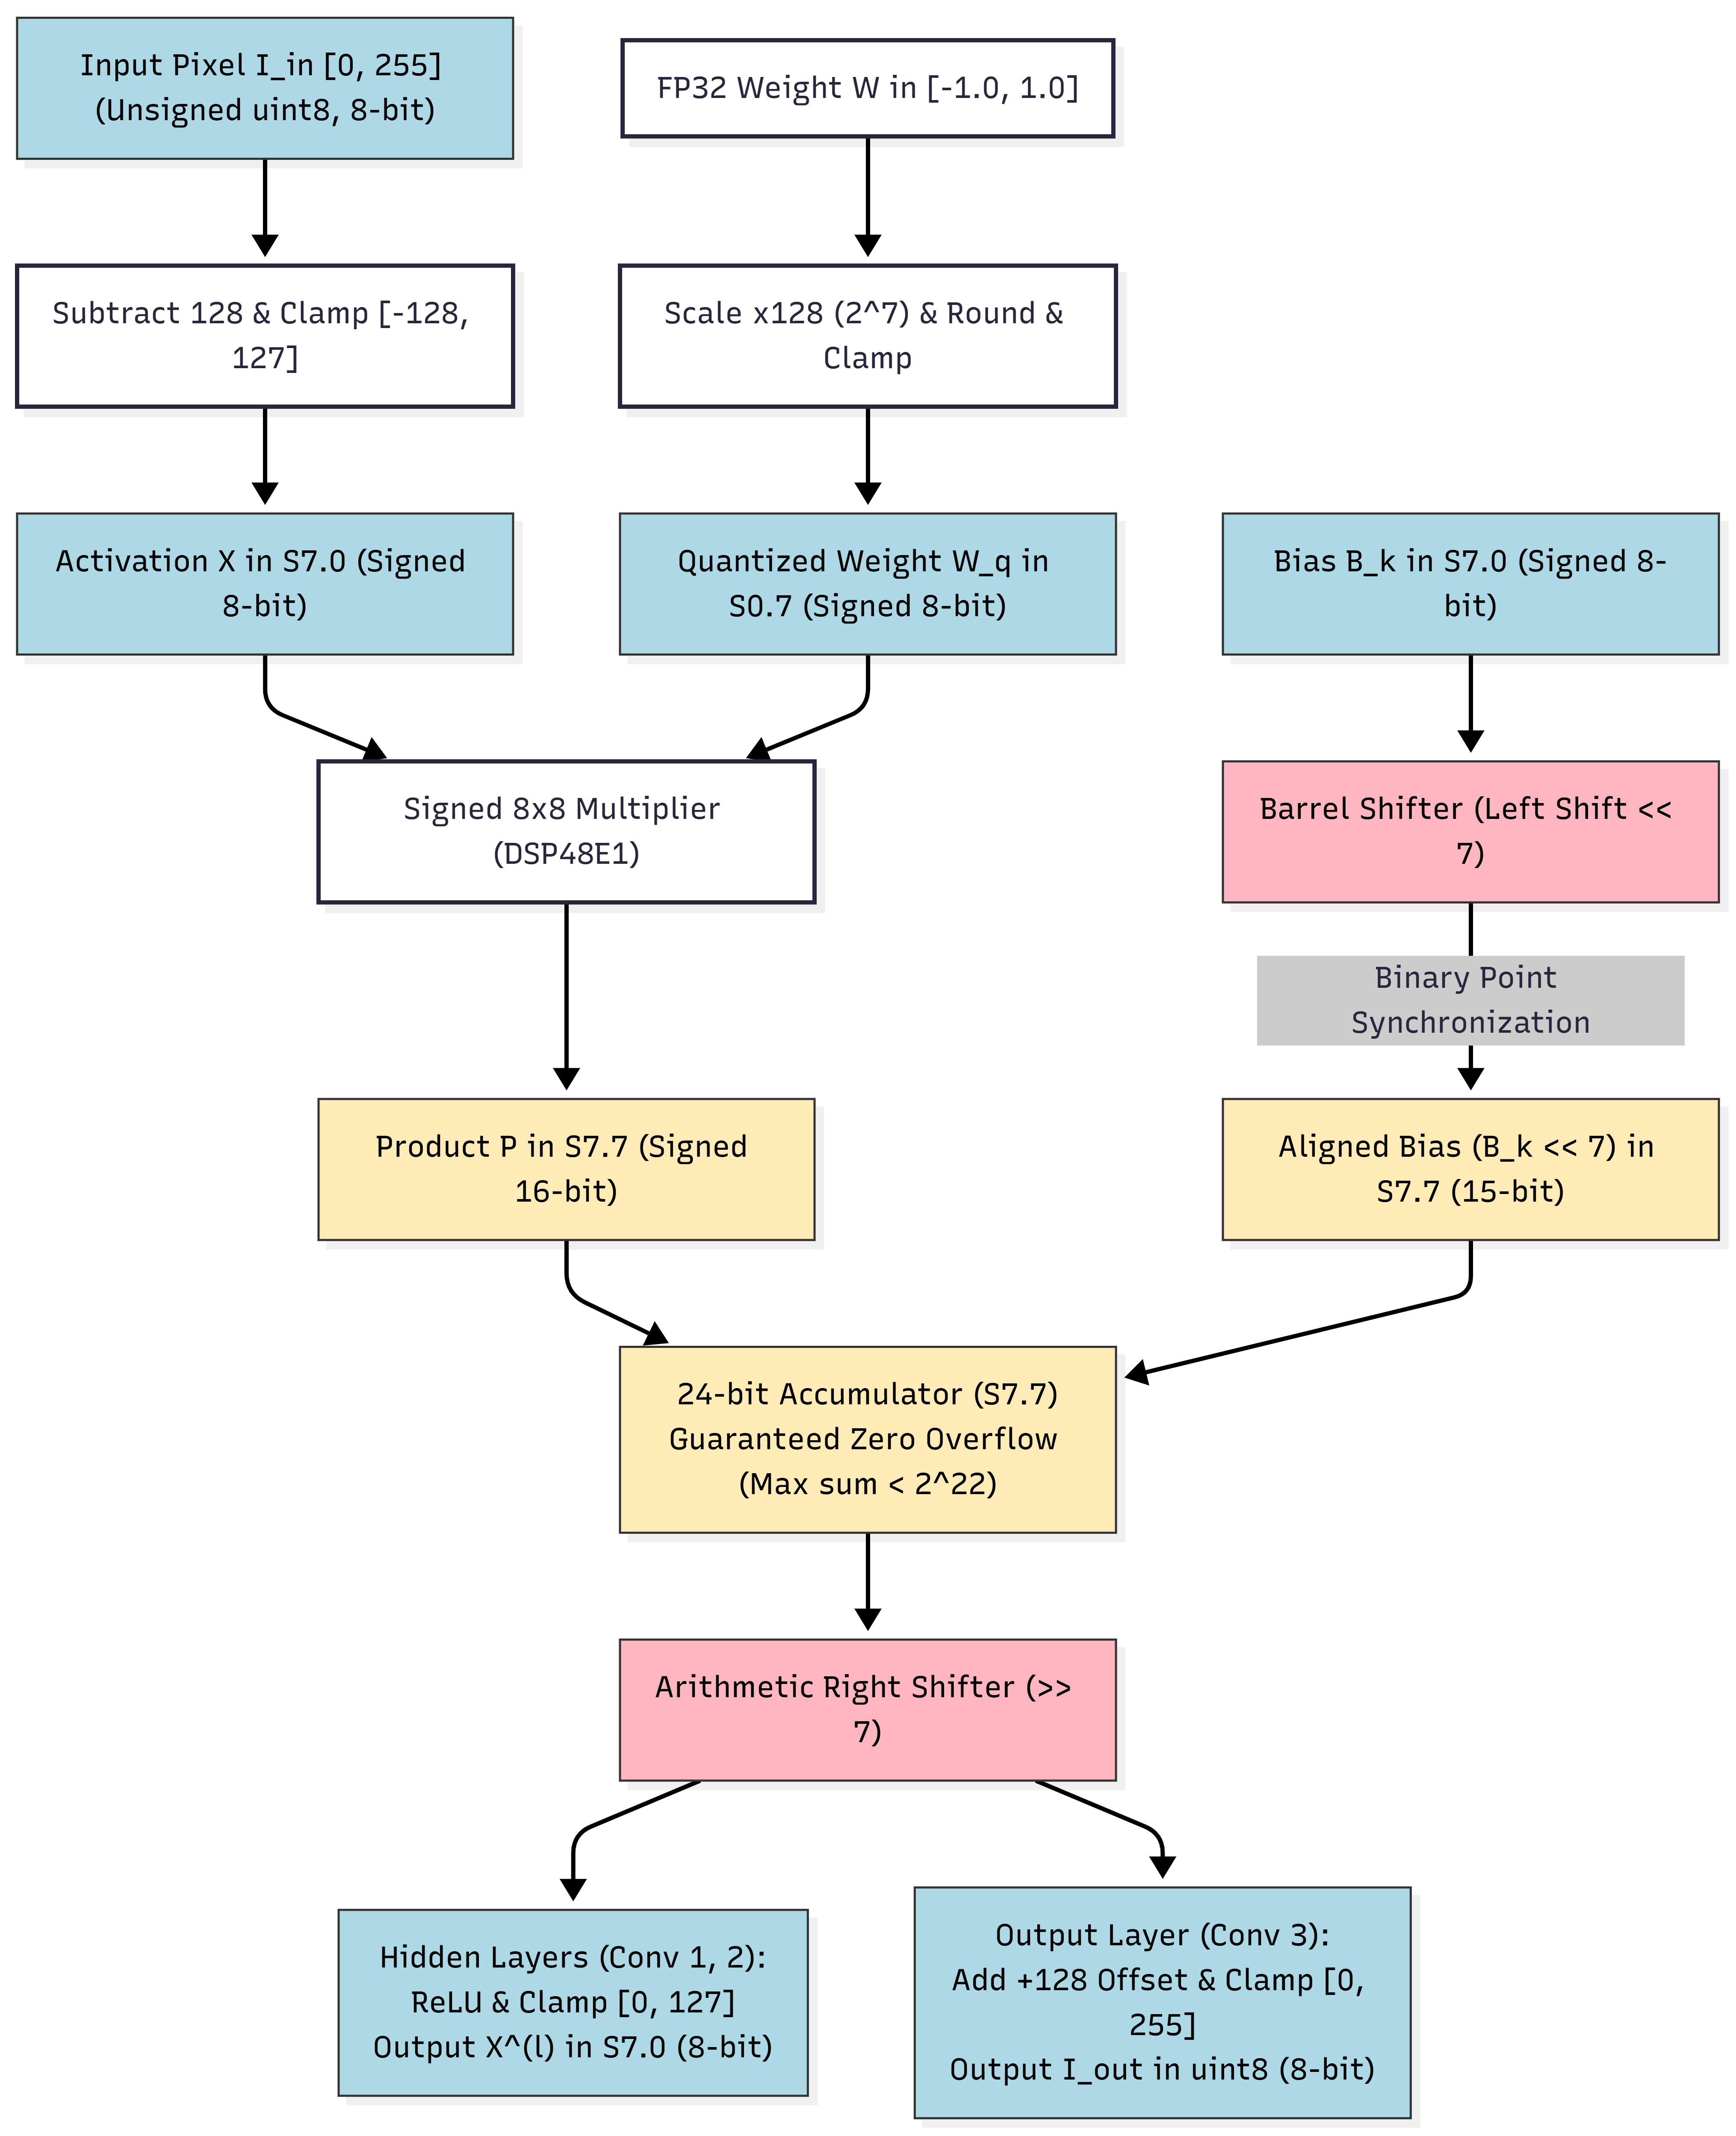
\includegraphics[width=\columnwidth]{fixed_point_datapath.png}
\caption{Hardware fixed-point arithmetic datapath and binary point alignment mechanism: (a) Input pixel conversion to signed S7.0, (b) Convolutional weight quantization into fractional S0.7, (c) Signed multiplication yielding intermediate S7.7 products, (d) Left bit-shifting of bias ($\ll 7$) for binary point synchronization before 24-bit accumulation, and (e) Arithmetic right-shifting ($\gg 7$) with ReLU and saturation clamping.}
\label{fig:fixed_point_datapath}
\end{figure}

\subsubsection{Input and Weight Quantization Mapping}
Raw grayscale radiographs are natively stored in unsigned 8-bit integer format ($I_{in} \in [0,\, 255]$). To leverage symmetrical 2's-complement arithmetic on DSP slices and eliminate asymmetrical zero-point offset computation in hardware, an offset of $-128$ is subtracted from each input pixel:
\begin{equation}
X^{(0)}(i, j) = \text{clamp}\left(I_{in}(i, j) - 128,\, -128,\, 127\right)
\label{eq:input_quant}
\end{equation}
where $\text{clamp}(x, a, b) = \min(\max(x, a), b)$. This transformation maps $[0,\, 255]$ symmetrically around zero to $[-128,\, 127]$, yielding the initial activation tensor $X^{(0)} \in \text{S7.0}$.

Continuous floating-point weights $W \in [-1.0,\, 1.0]$ are quantized into S0.7 integers by multiplying by scaling factor $2^7 = 128$, rounding to the nearest integer, and clamping against arithmetic saturation boundaries:
\begin{equation}
W_q = \text{clamp}\left(\left\lfloor W \cdot 2^7 \right\rceil,\, -128,\, 127\right)
\label{eq:weight_quant}
\end{equation}
where $\lfloor \cdot \rceil$ denotes round-to-nearest integer.

\subsubsection{Convolutional Accumulation and Binary Point Alignment}
A critical mathematical consideration in fixed-point arithmetic is the alignment of fractional radix points during Multiply-Accumulate (MAC) operations. Multiplying a signed activation $X \in \text{S7.0}$ by a signed weight $W_q \in \text{S0.7}$ produces an intermediate product $P = X \cdot W_q$ with $7 + 0 = 7$ fractional bits, occupying the \textbf{$\text{S7.7}$ format}. Mathematically, multiplying two signed 8-bit integers spans a 15-bit dynamic range ($[-16,384,\, +16,383]$); in the physical RTL implementation, this product is registered in a standard 16-bit signed two's-complement format (providing one sign-extension guard bit) to preserve byte alignment and match standard FPGA DSP output ports.

Because layer biases $B_k$ share the activation dynamic range and are natively quantized in S7.0 format, they cannot be directly added to the S7.7 product sum without inducing catastrophic scale misalignment. To synchronize binary points before accumulation, each bias term $B_k$ is bit-shifted left by 7 positions ($B_k \ll 7 = B_k \cdot 2^7$), lifting its representation into the S7.7 coordinate space. The unified MAC accumulation for output channel $k$ at coordinate $(i, j)$ is formulated as:
\begin{equation}
A_k(i, j) = \sum_{c=0}^{C_{in}-1} \sum_{u=0}^{K-1} \sum_{v=0}^{K-1} X_c(i+u, j+v) \cdot W_{k,c}(u, v) + \left(B_k \ll 7\right)
\label{eq:mac_accumulation}
\end{equation}
The complete hardware arithmetic datapath, including binary point synchronization, accumulation, and saturation clamping, is illustrated in Fig.~\ref{fig:fixed_point_datapath}.

To prevent arithmetic overflow during large spatial summations, the internal accumulator register bit-width is analyzed. In Layer~1 ($K = 9, C_{in} = 1$), the maximum theoretical sum over $9 \times 9 = 81$ products satisfies:
\begin{equation}
\max |A_k| \le 81 \times 128 \times 128 + 128 \times 128 = 1,343,488 < 2^{21}
\label{eq:accumulator_bound}
\end{equation}
Similarly, in Layer~3 ($K=5, C_{in}=8$), the maximum sum over $5 \times 5 \times 8 = 200$ products is bounded by $200 \times 128 \times 128 \approx 3.28 \times 10^6 < 2^{22}$. Consequently, sizing all internal accumulators to \textbf{24 bits} provides over 2 bits of guard margin, guaranteeing zero arithmetic overflow under all worst-case image patterns.

\subsubsection{Hidden Layer Activation, Re-Quantization, and Output Recovery}
To prepare intermediate feature maps for cascading into subsequent convolutional stages, the 24-bit accumulator value $A_k(i, j) \in \text{S7.7}$ must be downscaled back to S7.0 format. This re-quantization is executed through an arithmetic right-shift of 7 bits ($\lfloor A_k \gg 7 \rfloor$), effectively dividing by $2^7$ while truncating fractional bits. 

For hidden layers ($l \in \{1, 2\}$), non-linear activation and saturation clamping are integrated into a single hardware operation:
\begin{equation}
X_k^{(l)}(i, j) = \min\left(\max\left(0,\, \left\lfloor A_k(i, j) \gg 7 \right\rfloor\right),\, 127\right), \quad l \in \{1, 2\}
\label{eq:layer_activation}
\end{equation}
The inner $\max(0, \cdot)$ implements the ReLU activation function, whereas the outer $\min(\cdot, 127)$ clamps activations at $+127$, eliminating wrap-around overflow distortion.

Finally, at the reconstruction stage ($l = 3$), Layer~3 operates linearly without ReLU thresholding. The accumulator output $A_3(i, j)$ is arithmetic right-shifted by 7 bits, restored to the unsigned grayscale domain by adding the $+128$ DC offset, and saturated into the valid display range $[0,\, 255]$:
\begin{equation}
I_{out}(i, j) = \min\left(\max\left(0,\, \left\lfloor A_3(i, j) \gg 7 \right\rfloor + 128\right),\, 255\right)
\label{eq:output_dequant}
\end{equation}
Equations~\eqref{eq:input_quant}--\eqref{eq:output_dequant} establish an end-to-end fixed-point datapath that requires only integer adders, shifters, and DSP multiplier slices, completely bypassing the silicon and power cost of floating-point units.

\bibliographystyle{IEEEtran}
\bibliography{bib/references}
\end{document}
